\section{Einleitung}

\subsection{Motivation} \label{Motivation}

\begin{displayquote}
  \glqq Weltweit ist die Fleischerzeugung zwischen 2002 und 2012 um 23\% und in Deutschland um 29\% gestiegen. Die globalen Fleischexporte erhöhten sich im gleichen Zeitraum um 60\%, in Deutschland sogar um 124\%. Deutschland zählt sowohl beim Import als auch beim Export von Fleisch- und Fleischprodukten zu den bedeutendsten Handelsnationen weltweit.\grqq{}
\end{displayquote}

\begin{flushright}
  \citet{Efken2015}
\end{flushright}

Lebensmittelsicherheit ist strategisch für die Volksgesundheit und das Wohlbefinden einer Gesellschaft. Der öffentliche Druck auf Hersteller für eine ausreichende Kennzeichnung von Produkten und ihre Bestandteile wird stetig größer. Jeder Teil der Lieferkette ist in der Verpflichtung im Falle von Kontamination schnellstmöglich reagieren zu können. \citep{EPER2002}.

Vom Rohstofflieferanten bis zum Endkunden gibt es allein in Deutschland ein Netz von Marktteilnehmern mit erheblicher Größe. Knapp 150.000 Betriebe für die Rinder Mast und Milchproduktion, etwa 30.000 Betriebe im Bereich der Schweinehaltung und rund 60.000 Unternehmen für die Geflügelhaltung \citep{Efken2015}. Dabei existiert kein Standardverfahren zwischen diesen Marktteilnehmern zum Informationsaustausch für die Chargenrückverfolgung. In der Fleischwarenindustrie beispielsweise existieren weit über 140 unterschiedliche Austauschformate zwischen den Teilnehmern einzelner Lieferketten.

Zum jetzigen Zeitpunkt (Stand 2019) findet eine Chargenrückverfolgung daher fast ausschließlich durch einen Datei-Austausch bzw. eine zentrale Datenbank je Teilnehmer der Lieferkette statt. Dabei müssen Informationen für einen mehrstufigen Produktionsprozess bereitgestellt und verarbeitet werden \citep{Siepermann2015}.

Aus der geringen Umsatzrendite von -1\% bis +1,5\%  und den dadurch entstehnden Druck am Markt bestehen zu bleiben resultieren immer häufiger Unregelmäßigkeiten innerhalb der Lieferkette. Nur Betriebe in Österreich und Spanien können eine langfristige Rentabilität innerhalb des europäischen Marktes aufweisen \citep{Efken2015}. Ein Beispiel für die genannten Unregelmäßigkeiten ist der \glqq Pferdefleisch Skandal\grqq{} aus dem Jahr 2013, bei dem Fleischprodukte nachträglich neu etikettiert und dadurch in Produkten wie Lasagne oder Hamburger Patties weiterverarbeitet wurden \citep{Bundespartei}.

Informationen der Lieferkette und einzelner Chargen werden zentral je Hersteller oder Transportunternehmen gepflegt und sind dadurch nicht ausreichend vor Manipulation geschützt innerhalb der gesamten Lieferkette. Die \textit{Blockchain-Technologie} ermöglicht das manipulationssichere ablegen von solchen Informationen und könnte daher eine Lösung für dieses Problem darstellen. Bereits heute gibt es Anwendungen der \textit{Blockchain}, um beispielsweise den Kilometerstand eines Fahrzeugs täglich \glqq in die \textit{Blockchain}\grqq{} zu schreiben. Die inhärenten Eigenschaften der \textit{Blockchain} ermöglichen es sehr einfach festzustellen, ob ein Kilometerstand nachträglich durch Fremdeinwirkung manipuliert wurde. Ebenfalls ist keine zentrale \glqq Clearing Stelle\grqq{} mehr nötig, um die Echtheit des hinterlegten Wertes sicherzustellen \citep{carVertical}.

\begin{figure}[H]
	\centering
	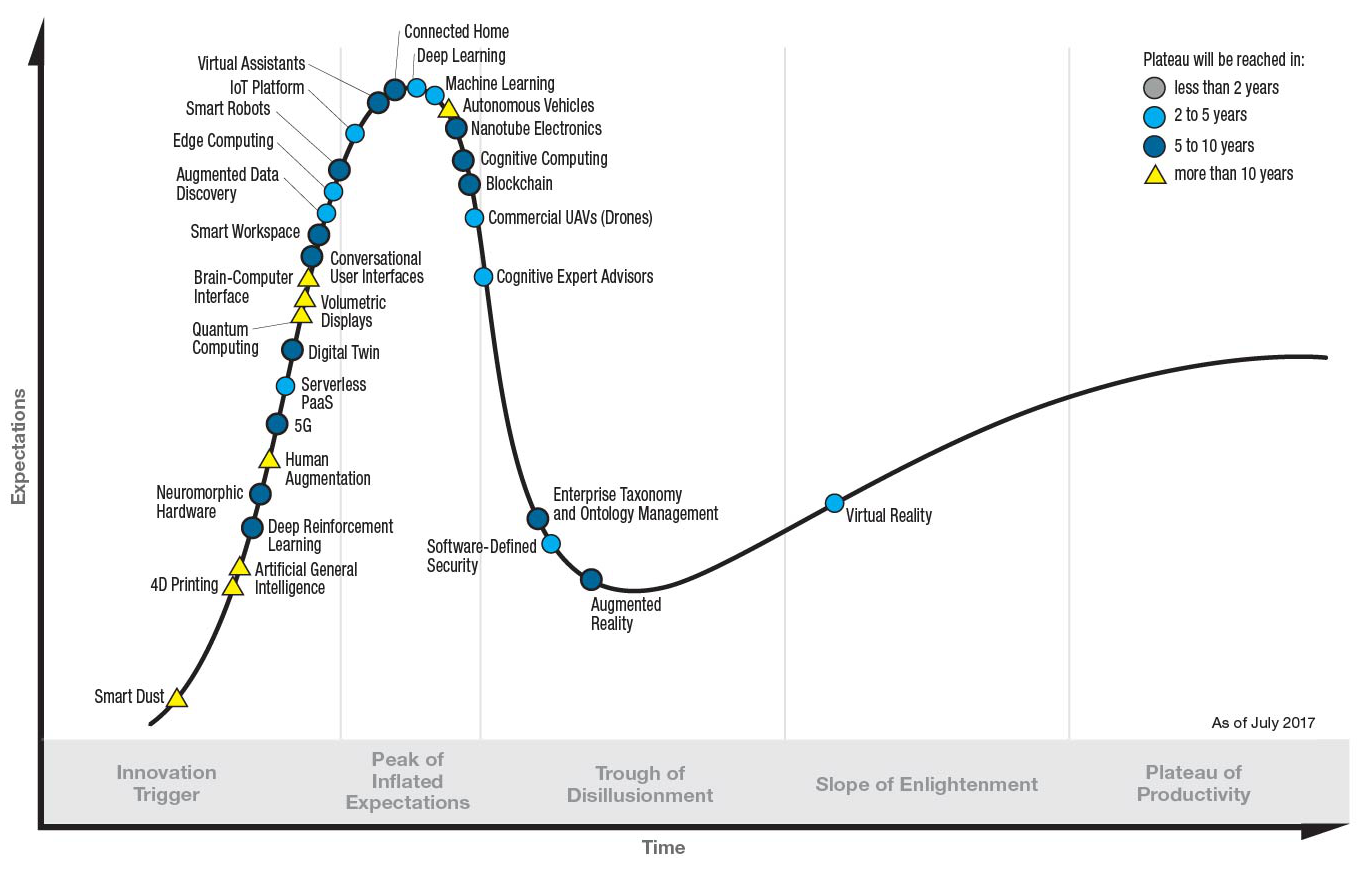
\includegraphics[width=1.0\linewidth]{pictures/Gartner-Hype-Cycle-2017}
	\caption[Gartner Hype Cycle 2017]{Emerging Technologies Hype Cycle 2017\citep{Gartner2017}}
	\label{fig:gartner-hype-cycle-2017}
\end{figure}

Aktuell ist die \textit{Blockchain} jedoch noch kein industrieller Standard oder verbreitet im Einsatz. Bemessen am jährlich erscheinenden Hype Cycle des Marktforschungsinstituts Gartner, Inc. $( Abb.~ \ref{fig:gartner-hype-cycle-2017} )$ hat die Technologie noch fünf bis zehn Jahre Entwicklungszeit vor sich. Erst dann wird sie nach aktueller Einschätzung im produktiven Einsatz sein.

\glqq Es ist davon auszugehen, dass wir in ein bis zwei Jahrzehnten wirtschaftlich über Mechanismen miteinander interagieren werden, für die wir bislang weder Konzepte noch Begriffe haben\grqq{} \citep[S.~92]{Platzer2014}.
Auch die Deutsche Bundesregierung ist an der \textit{Blockchain-Technologie} interessiert und erwägt den Einsatz in Zukunft für die unterschiedlichsten Services. In einer der jüngsten Pressemitteilungen hat der \textit{Blockchain} Bundesverband mitgeteilt, dass die Regierung eine umfassende Strategie zum Umgang und Einsatz der Technologie erarbeiten will \citep{BCBundesverband2018}.

\subsection{Problemstellung} \label{Problemstellung}

Um eine formal korrekte Identitätskette vom Erzeuger bis zum Groß- und Einzelhandel aufzubauen, wird eine verlässliche Basis, grade auch dann, wenn Futtermittel- und Logistik-Informationen unter allen Marktteilnehmern ausgetauscht werden müssen, benötigt. Grundlage dafür ist die EU-Verordnung 178/02 (insbesondere Artikel 18 und 19), welche die Notwendigkeit beschreibt, dass jeder Akteur der Lieferkette dafür verantwortlich ist, nachzuweisen von wem er seine Waren bezogen und an wen er seine Waren geliefert hat \citep{EPER2002}.

% Aktuelle Lösung beim Praxispartner erläutern und auf Probleme hinweisen!
Als konkretes Beispiel wird beim Praxispartner Westfleisch SCE mbH zur Realisierung einer Chargenrückverfolgung die Software \ac{gbt} vom Hersteller SAP eingesetzt. Mithilfe dieser Software werden die Stammdatenobjekte \textit{Charge}, \textit{Produkt} und \textit{Geschäftspartner} verwaltet und mit dem \ac{erp} System integriert. \ac{gbt} ist dabei als zentrales System konzipiert, welches über eine Schnittstelle von Akteuren der Lieferkette mit Informationen zu einer \textit{Charge} beliefert werden kann. Diese Schnittstelle verwendet \textit{\acs{idoc}}\footnote{Ein \ac{idoc} ist ein Container für den Datenaustausch zwischen SAP und Nicht-SAP-Systemen \citep{SAP2019}.} bzw. \textit{\acs{xml}}\footnote{Die \ac{xml} ist eine Auszeichnungssprache zur Darstellung hierarchisch strukturierter Daten im Format einer Textdatei \citep{Yergeau2008}.} als Austauschformat. Der eigentliche Austausch erfolgt dabei entweder manuell über einen Dateiimport/-export Mechanismus oder über das Internet mittels des \textit{\acs{http}}\footnote{\ac{http}} Protokolls. Bei diesem Austausch besteht grundsätzlich die Möglichkeit, dass Datensätze vor dem Austausch oder nachträglich verändert werden können - ohne das Teilnehmer der Lieferkette hiervon etwas mitbekommen würden.\\

Aus den beschriebenen Sachverhalten ergibt sich für eine zeitnahe und transparente Rückverfolgung von \textit{Chargen} über den gesamten Verlauf der Wertschöpfungskette in Produktionsnetzwerken mittels \textit{Blockchain-Technologie} folgende Forschungsfrage:

\begin{itemize}
  \item[\textbf{FF1}] \textbf{Wie kann die Rückverfolgbarkeit von \textit{Chargen} in der Fleischwarenindustrie entlang der gesamten Lieferkette mithilfe von \textit{Blockchain-Technologie} realisiert werden?}
  \begin{itemize}
    \item[FF1.1] Welche Anforderungen an ein System zur Rückverfolgbarkeit von \textit{Chargen} werden seitens der Fleischwarenindustrie gestellt?
    \item[FF1.2] Welche Daten müssen in einer \textit{Blockchain} persistiert werden, um eine Rückverfolgbarkeit zu ermöglichen?
    \item[FF1.3] Welche \textit{Blockchain-Technologie} kommt in Frage um FF1 zu realisieren und den spezifischen Anforderungen der Fleischwarenindustrie gerecht zu werden?
    \item[FF1.4] Welche Systemarchitektur erfüllt die Anforderungen der Fleischwarenindustrie, um eine Chargenrückverfolgung zu realisieren?
    % \item[FF1.4] Wie könnte eine Systemarchitektur für ein durch \textit{Blockchain-Technologie} gestütztes System konzipiert sein?
  \end{itemize}
\end{itemize}

\subsection{Vorgehen / Methodik}

Die in Abschnitt \ref{Problemstellung} beschriebenen Probleme und Herausforderungen sollen gelöst werden mittels der Design Science Methode nach \citet{Hevner2004, Hevner2007}. Dabei konzentriert sich Design Science auf die Entwicklung von (entworfenen) Artefakten mit der Absicht, die funktionale Leistung des Artefakts zu verbessern. Design Science wird in der Regel für Artefakte aus den Kategorien Algorithmen, Mensch-Computer-Schnittstellen und Prozessmodellen verwendet \citep{Peffers2012, Kuechler2008}. Abbildung \ref{fig:three-cycles-design-science} stellt die drei Design Science Zyklen nach \citet{Hevner2010} dar.

\begin{figure}[h!]
	\centering
	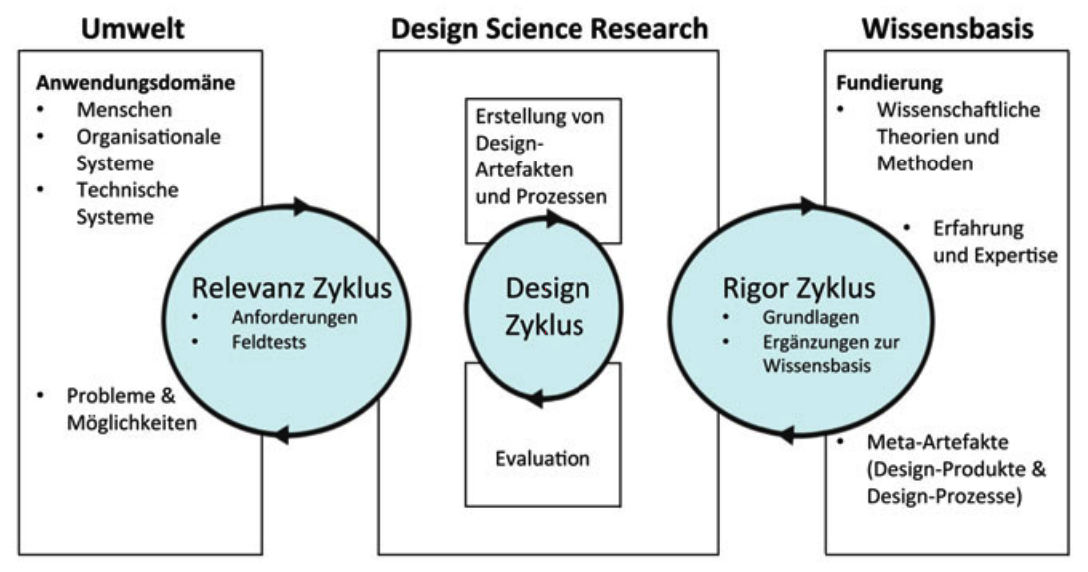
\includegraphics[width=1.0\linewidth]{pictures/three-cycles-design-science}
	\caption[Die drei Design Science Zyklen nach Hevner]{Die drei Design Science Zyklen nach \citet{Hevner2010} \citep{Trepper2015}}
	\label{fig:three-cycles-design-science}
\end{figure}

Im Sinne des Relevanz Zyklus \citep[siehe auch][]{Simon1996} soll eine Betrachtung der bisherigen Supply Chain Systeme und der Wertschöpfungskette inklusive ihrer einzelnen Geschäftsprozesse aus technischer Sicht erfolgen. Als Ergebnis dieser Betrachtung sollen Anforderungen an das Artefakt identifiziert werden. Anschließend wird durch den Rigor Zyklus eine wisschenschaftliche Basis erarbeitet, um bereits vorhandene Erkenntnisse in die Arbeit einfließen zu lassen. Durch den Rigor Zyklus soll sichergestellt werden, dass das Artefakt eine Innovation darstellt und nicht bereits erforschte Resultate repliziert werden \citep{Hevner2010}. Innerhalb des Design Zyklus soll ein möglicher Systementwurf zur Lösung der Probleme aus Abschnitt \ref{Problemstellung} erarbeitet werden. Dieser Systementwurf wird als Prototyp implementiert und anschließend einer Evaluation durch Experteninterviews \citep[siehe auch][]{Wilde2007} unterzogen.

\subsection{Ziele}

Der Einsatz von \textit{Blockchain-Technologie} könnte - für die in Kapitel \ref{Problemstellung} beschriebene Problemstellung - eine Lösung darstellen. Eine \textit{Blockchain} ist ein dezentrales System zur manipulationssicheren Speicherung von Informationen in sog. \textit{Blöcken} die untereinander durch kryptographische Methoden verkettet sind - daher auch der Name \textit{Blockchain}. Eine \textit{Blockchain} verwendet verschiedenste Verfahren zur Konsensbildung innerhalb des Netzwerks, um sicherzustellen das neue \textit{Blöcke} und die darin enthaltenen Transaktionen vom gesamten Netzwerk validiert und verifizert werden bevor der \textit{Block} in die \textit{Blockchain} geschrieben wird \citep[siehe auch][]{Nakamoto2009, Buterin2014, Cardano2017, carVertical}.

Außerdem kann eine \textit{Blockchain} durch den Einsatz einer kryptographischen \textit{Hashfunktion}\footnote{Spezielle Form einer Hashfunktion, welche kollisionsresistent ist. Es ist praktisch nicht möglich, zwei unterschiedliche Eingabewerte zu finden, die einen identischen Hashwert ergeben \citep{Menezes1997}.} zur Bildung einer Prüfsumme für jeden \textit{Block} innerhalb der \textit{Blockchain} sicherstellen, dass bereits persistierte Informationen nicht ohne weiteres manipuliert werden können. Im Idealfall ist eine \textit{Blockchain} dezentral konzipiert, was bedeutet, das jeder Teilnehmer eines \textit{Blockchain} Netzwerks eine exakte Kopie des Datenbestands lokal vorhält. Hierdurch soll sichergestellt werden, das auch bei einem Ausfall oder einer Kompromittierung einzelner Teilnehmer das Gesamtsystem weiterhin in seiner Funktion stabil bleibt \citep{Drescher2017, Tribis2018}.\\

Ziel dieser Arbeit ist es, durch Entwicklung und Evaluation eines Prototyps die Möglichkeiten und Grenzen der \textit{Blockchain-Technologie} im Kontext der Chargenrückverfolgung in der Fleischwarenindustrie zu überprüfen. Dabei sollen die dafür nötigen Daten und Informationen ermittelt und in einen Systementwurf eingearbeitet werden. Außerdem ist angestrebt, aus der Vielzahl von unterschiedlichen Implementierungen einer \textit{Blockchain} genau die Ausprägung zu identifizieren, welche für die spezifischen Anforderungen der Fleischwarenindustrie ideal erscheint.

Konkret lassen sich hieraus folgende Ziele und erwartete Ergebnisstypen zu den jeweiligen Forschungsfragen aus Kapitel \ref{Problemstellung} ableiten:

\begin{itemize}
  \item Identifikation verwandter Arbeiten aus Wissenschaft und Praxis für FF1.1
  \item Anforderungserhebung und -analyse mit dem Praxispartner für FF1.1
  \begin{itemize}
    \item Funktional
    \item Qualitativ
    \item Rahmenbedingungen
  \end{itemize}
  \item Prozessaufnahme und -analyse für FF1.2
  \begin{itemize}
    \item Schwachstellenanalyse des \textit{Ist}-Prozess
    \item Modellierung eines \textit{Soll}-Prozess bei Einsatz von \textit{Blockchain-Technologie}
  \end{itemize}
  \item SWOT-Analyse als Vorbereitung für eine Nutzwertanalyse zur Klärung von FF1.3
  \item Ableitung eines Systementwurfs mittels Design Science Research für FF1.4
  \item Entwicklung eines Prototyps anhand der Ergebnisse von FF1.1-4 für FF1
  \item Evaluation des Prototyps durch Experteninterview für FF1
\end{itemize}

Der enstandene Prototyp soll beim Praxispartner Westfleisch SCE mbH in Münster/Coesfeld als Entscheidungshilfe für eine zukünftige Innovationsstrategie zur Optimierung der Lieferkette dienen.

\subsection{Struktur der Arbeit}

\textcolor{red}{Lorem ipsum dolor sit amet, consetetur sadipscing elitr, sed diam nonumy eirmod tempor invidunt ut labore et dolore magna aliquyam erat, sed diam voluptua. At vero eos et accusam et justo duo dolores et ea rebum. Stet clita kasd gubergren, no sea takimata sanctus est Lorem ipsum dolor sit amet. Lorem ipsum dolor sit amet, consetetur sadipscing elitr, sed diam nonumy eirmod tempor invidunt ut labore et dolore magna aliquyam erat, sed diam voluptua. At vero eos et accusam et justo duo dolores et ea rebum. Stet clita kasd gubergren, no sea takimata sanctus est Lorem ipsum dolor sit amet.}

\newpage
